\documentclass[11pt,addpoints]{exam}
\usepackage{amsfonts,amssymb,amsmath, amsthm}
\usepackage{graphicx}
\usepackage{systeme}
\usepackage{pgf,tikz,pgfplots}
\pgfplotsset{compat=1.15}
\usepgfplotslibrary{fillbetween}
\usepackage{mathrsfs}
\usetikzlibrary{arrows}
\usetikzlibrary{calc}
\usepackage{enumitem}
\usepackage{multicol}


\pagestyle{headandfoot}
\firstpageheader{AP Calc. AB - Exam 2 Practice Problems\\ Exam date: August 24}{}{Name: \underline{\hspace{2.5in}}}
\runningheader{AP Calc. AB - Exam 2 Practice Problems}{}{Page \thepage\ of \numpages}
\runningheadrule
\firstpagefooter{}{}{}
\runningfooter{}{}{}
\begin{document}
\begin{questions}
    \question For each circle, find its (i) center, (ii) radius, and (iii) equation for the (left/right/top/bottom) specified semicircle.
    \begin{parts}
        \part $x^2 - 12x + y^2 - 4y = -15$
        \part $x^2 + y^2 + 6x + 6y = 31$
        \part $4x + y^2 + x^2 = 45$
    \end{parts}
    
    \question Sketch each solution set:
    \begin{multicols}{2}
        \begin{parts}
            \part $\{(x,y)\mid|x| < 4\text{, }y > 3\}$
            \part $\{(x,y)\mid x^2 + (y-1)^2 \leq 16\}$
            \part $\{(x,y)\mid y \geq \frac{2}{3}x - 2\}$
            \part $\{(x,y)\mid x^2 - 2x + 1 \geq y\text{, }y > -4\}$
            \part $\{(x,y)\mid y \leq x^2 + 2x - 3\text{, }|x| < 4\}$
            \part $\{(x,y)\mid y \leq \sqrt{x}\text{, }y \geq 0\text{, }x<3\}$
        \end{parts}
    \end{multicols}
    
    \question Evaluate:
    \begin{multicols}{2}
        \begin{parts}
            \part $\tan\left(\frac{2\pi}{3}\right)$ % = -sqrt(3)
            \part $\csc\left(\frac{\pi}{2}\right)$ % = 1
            \part $\sin\left(-\frac{\pi}{4}\right)$ % = 
            \part $\cot\left(\frac{5\pi}{6}\right)$ % = 
            \part $\cos\left(3\pi\right)$ % = 
            \part $\sec\left(-\frac{2\pi}{3}\right)$ % = 
            \part $\sin\left(\frac{3\pi}{4}\right)$ % = 
            \part $\tan\left(-\pi\right)$ % = 
            \part $\cos\left(\frac{7\pi}{2}\right)$ % = 
            \part $\csc\left(-\frac{\pi}{3}\right)$ % = 
            \part $\sec\left(\frac{\pi}{4}\right)$ % = 
            \part $\cot\left(\frac{\pi}{3}\right)$ % = 
        \end{parts}
    \end{multicols}

    \question This question has multiple sections: (a)-(d), sketch the piecewise-defined function; (e)-(h), rewrite each function as a piecewise one; (i)-(k), find piecewise formulas for each graph.
    \begin{multicols}{2}
        \begin{parts}
            \part$
                f(x) =
                \begin{cases}
                    -1 & \text{if } x < -1\\
                    0 & \text{if } -1 \leq x \leq 0\\
                    1 & \text{if } 0 < x \leq 1\\
                    2 & \text{if } x > 1
                \end{cases}
            $ % https://www.desmos.com/calculator/ukc49papmx
            \part$
                f(x) =
                \begin{cases}
                    x+2 & \text{if } x < 1\\
                    -x^2+4 & \text{if } x \geq 1
                \end{cases}
            $ % https://www.desmos.com/calculator/ngaiihowvp
            \part$
                f(x) =
                \begin{cases}
                   0 & \text{if } x < 0\\
                   x & \text{if } 0 \leq x < 3\\
                   -2x+9 & \text{if } x > 3
                \end{cases}
            $ % https://www.desmos.com/calculator/anjf30i9sp
            \part$
                f(x) =
                \begin{cases}
                   (x+1)^2-3 & \text{if } x < 0\\
                   -\frac{1}{2}x-2 & \text{if } 0 \leq x < 2\\
                   2x-7 & \text{if } x \geq 2
                \end{cases}
            $ % https://www.desmos.com/calculator/2hciari9qc
        \end{parts}
    \end{multicols}
    \vspace*{0.1cm}
    \begin{multicols}{2}
        \begin{parts}
            \setcounter{partno}{4}
            \part $f(x) = |1-2x|$
            \part $f(x) = -|3x+2|+4$
            \part $f(x) = -|-x+2|-1$
            \part $f(x) = |x|-|x+1|$
        \end{parts}
    \end{multicols}
    \vspace*{0.1cm}
    \begin{parts}
        \setcounter{partno}{8}
        \begin{multicols}{3}
            \part{
                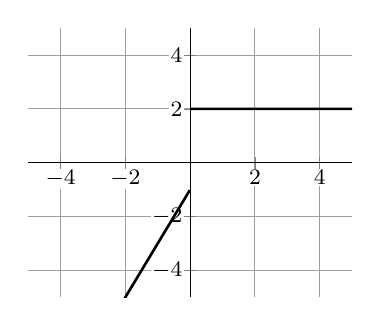
\begin{tikzpicture}[declare function={g(\x)=\x<0 ? 2*\x-1 : (\x>0 ? 2 : inf);}]
        			\begin{axis}[unbounded coords=jump,
        					grid=both,
        					grid style={line width=0.35pt, draw=gray!75},
        					axis lines=center,
        					axis line style={-},
        					xmin=-5, xmax=5,
        					ymin=-5, ymax=5,
        					ticklabel style={font=\footnotesize,inner sep=0.5pt,fill=white,opacity=1.0, text opacity=1},
        					every axis plot/.append style={line width=0.95pt, color=black, samples=500},
        					scale=0.6
        				]
        				\addplot[samples at={-5,-0.01,0,0.01,5}] {g(x)};
        			\end{axis}
        		\end{tikzpicture}
            }
            \part{
                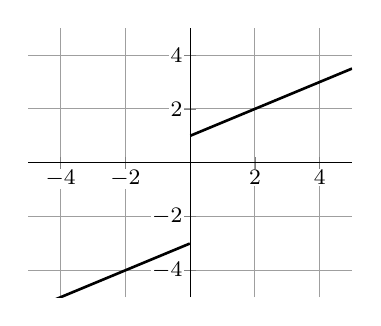
\begin{tikzpicture}[declare function={g(\x)=\x<0 ? 1/2*x-3 : (\x>0 ? 1/2*x+1 : inf);}]
        			\begin{axis}[unbounded coords=jump,
        					grid=both,
        					grid style={line width=0.35pt, draw=gray!75},
        					axis lines=center,
        					axis line style={-},
        					xmin=-5, xmax=5,
        					ymin=-5, ymax=5,
        					ticklabel style={font=\footnotesize,inner sep=0.5pt,fill=white,opacity=1.0, text opacity=1},
        					every axis plot/.append style={line width=0.95pt, color=black, samples=500},
        					scale=0.6
        				]
        				\addplot[samples at={-5,-0.01,0,0.01,5}] {g(x)};
        			\end{axis}
        		\end{tikzpicture}
            }
            \part{
                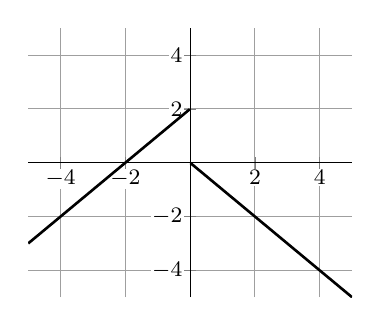
\begin{tikzpicture}[declare function={g(\x)=\x<0 ? x+2 : (\x>0 ? -x : inf);}]
        			\begin{axis}[unbounded coords=jump,
        					grid=both,
        					grid style={line width=0.35pt, draw=gray!75},
        					axis lines=center,
        					axis line style={-},
        					xmin=-5, xmax=5,
        					ymin=-5, ymax=5,
        					ticklabel style={font=\footnotesize,inner sep=0.5pt,fill=white,opacity=1.0, text opacity=1},
        					every axis plot/.append style={line width=0.95pt, color=black, samples=500},
        					scale=0.6
        				]
        				\addplot[samples at={-5,-0.01,0,0.01,5}] {g(x)};
        			\end{axis}
        		\end{tikzpicture}
            }
        \end{multicols}
    \end{parts}
    \question For each of the following functions, evaluate the difference quotient: \[\frac{f(x+h)-f(x)}{h}\]
    \begin{multicols}{3}
        \begin{parts}
            \part $f(x) = x^2 + 3$
            \part $f(x) = 2x^3 + 7$
            \part $f(x) = 4x^2 + 2x + 9$
        \end{parts}
    \end{multicols}
\end{questions}
\end{document}